\begin{enumerate}[label=\thechapter.\arabic*,ref=\thechapter.\theenumi]

\item The number of zeroes of the polynomial $P(s) = s^3+2s^2+5s+80$ in the right side of the plane?\hfill(GATE IN 2023) \\

\solution
\iffalse
\let\negmedspace\undefined
\let\negthickspace\undefined
\documentclass[journal,12pt,twocolumn]{IEEEtran}
\usepackage{cite}
\usepackage{amsmath,amssymb,amsfonts,amsthm}
\usepackage{algorithmic}
\usepackage{graphicx}
\usepackage{textcomp}
\usepackage{xcolor}
\usepackage{txfonts}
\usepackage{listings}
\usepackage{enumitem}
\usepackage{mathtools}
\usepackage{gensymb}
\usepackage{comment}
\usepackage[breaklinks=true]{hyperref}
\usepackage{tkz-euclide} 
\usepackage{listings}
\usepackage{gvv} 
\usepackage{caption}
\def\inputGnumericTable{}                   

%\usepackage[latin1]{inputenc}                                
\usepackage{color}                                            
\usepackage{array}                                            
\usepackage{longtable}                                       
\usepackage{calc}                                             
\usepackage{multirow}                                         
\usepackage{hhline}                                           
\usepackage{ifthen}                                           
\usepackage{lscape}

\newtheorem{theorem}{Theorem}[section]
\newtheorem{problem}{Problem}
\newtheorem{proposition}{Proposition}[section]
\newtheorem{lemma}{Lemma}[section]
\newtheorem{corollary}[theorem]{Corollary}
\newtheorem{example}{Example}[section]
\newtheorem{definition}[problem]{Definition}
\newcommand{\BEQA}{\begin{eqnarray}}
\newcommand{\EEQA}{\end{eqnarray}}
\newcommand{\define}{\stackrel{\triangle}{=}}
\theoremstyle{remark}
\newtheorem{rem}{Remark}

\begin{document}

\bibliographystyle{IEEEtran}
\vspace{3cm}

\title{GATE: IN - 24.2023}
\author{EE23BTECH11013 - Avyaaz$^{*}$% <-this % stops a space 
}
\maketitle
\newpage
\bigskip

\renewcommand{\thefigure}{\arabic{figure}}
\renewcommand{\thetable}{\arabic{table}}

\large\textbf{\textsl{Question:}}
The number of zeroes of the polynomial $P(s) = s^3+2s^2+5s+80$ in the right side of the plane?\hfill(GATE IN 2023) \\
\solution
\fi
The table below shows the Routh array of the $n^{th}$- order characteristic polynomial : 
\begin{align}
    a_0s^n+a_1s^{n-1}......+a_{n-1}s^1+a_ns^0
\end{align}

\begin{table}[htbp]
\setlength{\extrarowheight}{8pt}
\centering
\begin{tabular}{|c|c|c|c|c|}
\hline 
$s^n$ & $ a_0 $ & $a_2 $ &  $a_4$ & ... \\
\hline
$s^{n-1}$ &$a_1$&$a_3$&$a_5$&...  \\
\hline
$s^{n-2} $& $b_1 = \dfrac{a_1a_2-a_3a_0}{a_1}$ &$b_2 = \dfrac{a_1a_4 - a_5a_0}{a_1}$ &...&..\\
\hline
$s^{n-3} $& $c_1 = \dfrac{b_1a_3-b_2a_1}{b_1}$  & $\vdots$ && \\
\hline
$\vdots$ & $\vdots$ & $\vdots$&&\\
\hline
$s^1$&$\vdots$&$\vdots$&&\\
\hline
$s^0$&$a_n$&&&\\
\hline
\end{tabular}

\caption{Routh Array}
\label{tab:routharray.IN.24.2023}
\end{table}
 Characteristic Equation:
\begin{align}
   s^3+2s^2+5s+80 = 0  
\end{align}


\noindent From \tabref{tab:routharray.IN.24.2023}:

\begin{table}[htbp]
\setlength{\extrarowheight}{10pt}
\centering
\begin{tabular}{|c|c|c|}
\hline 
$s^3$ & $ 1 $ & $5$ \\
\hline
$s^2$ &$2$&$80$ \\
\hline
$s^1 $& $\dfrac{2\times 5-80\times1}{2}= 
 -35$ & \\
\hline
$s^0 $& $ \dfrac{-35 \times 80}{-35} = 80$ &\\
\hline
\end{tabular}

\caption{}
\label{tab:inputs.IN.24.2023}
\end{table}

% The number of sign changes of the terms of the first column of the Routh Array corresponds to the number of roots of the characteristic equation in the right half of the s-plane.

\noindent From \tabref{tab:inputs.IN.24.2023}:

Since there are 2 sign changes in the first column of the Routh tabulation. So, the number of zeros in the right
half of the s-plane will be 2.

% s1 = -4.63925
% s2 = 1.31963 + 3.93735 i
% s3 = 1.31963 - 3.93735 i
% A pole is a value of s (in the Laplace domain) for which the transfer function becomes infinite.
% A zero is a value of s for which the transfer function becomes zero.

% In the Laplace domain, a transfer function 
% H(s) is typically represented as a ratio of polynomials in s: H(s)= N(s)/D(s)

\begin{figure}[htbp]
    \centering
    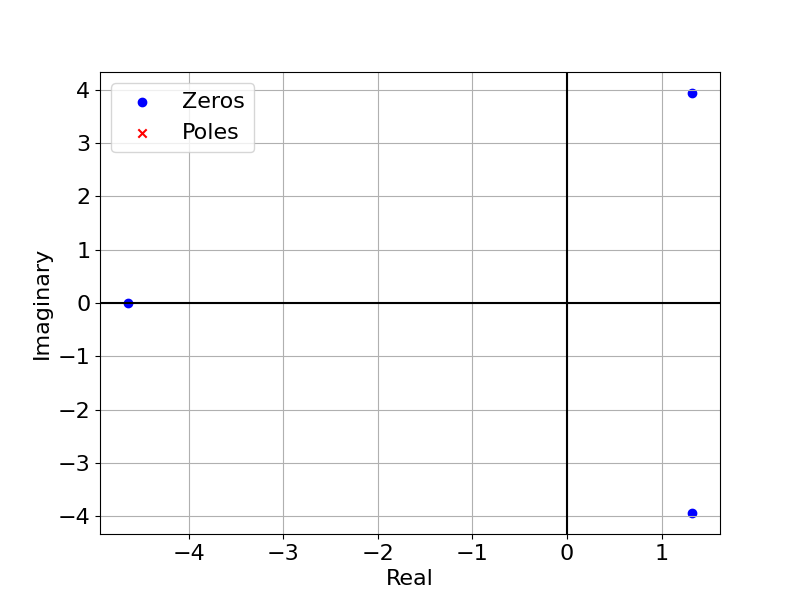
\includegraphics[width = \columnwidth]{2023/IN/24/figs/poles and root_plot.png}
  \caption{}
    \label{fig:graph1}
\end{figure}

% \bibliographystyle{IEEEtran}

\newpage

\item The circuit shown in the figure is initially in the steady state with the switch K in open condition and $\overline{K}$ in closed condition. The switch K is closed and $\overline{K}$ is opened simultaneously at the instant $t = t_1$, where $t_1 > 0$. The minimum value of $t_1$ in milliseconds such that there is no transient in the voltage across the 100 $\mu F$ capacitor, is \rule{1cm}{0.15mm} (Round off to 2 decimal places) \hfill (GATE EE 2023)
    \begin{circuitikz}[american]
        \draw (0,7) to [R=10$\Omega$] (0,2) to [short] (3.5,2) to [isource, l={$\sin\brak{1000t}$}] (3.5,7) to [short] (0,7);
        \draw (3.5,2) to [short] (5,2) to [short] (5,0) to [R=$10\Omega$] (7.5,0) to [battery2 = 5V] (10,0) to [short] (10,2) to [curved capacitor=100$\mu$F, invert] (10,7) to [short] (5,7) to [short] (3.5,7);
        \draw (5,2) to [short] (7, 2) to[ospst=$\overline{K}$] ++(1,0);
        \draw (5,5) to [short] (5,2);
        \draw (10,2) to [short] (8,2);
        \draw (5,7) to [short] (5,6) to[cspst=K] ++(0,-1) ;
\end{circuitikz}


\newpage
\item $y=e^{mx}+e^{-mx}$ is the solution of which differential equation?
\begin{enumerate}[label=\textbf{\arabic*.}, font=\bfseries, align=left]
    \item $\frac{dy}{dx} - my = 0$ 
    \item $\frac{dy}{dx} + my = 0$ 
    \item $\frac{d^{2}y}{dx^{2}} + m^{2}y = 0$ 
    \item $\frac{d^{2}y}{dx^{2}} - m^{2}y = 0$ 
\end{enumerate} \hfill(GATE AG 2023)
\solution

\newpage
\item  A cascade control strategy is shown in the figure below. The transfer function between the output $(y)$ and the secondary disturbance $(d_2)$ is defined as  \\
$$G_{d2}(s)= \frac{y(s)}{d_2(s)}$$. 
Which one of the following is the CORRECT expression for the transfer function $G_{d2}(s)$? \\
\begin{figure}[h]
    \centering
    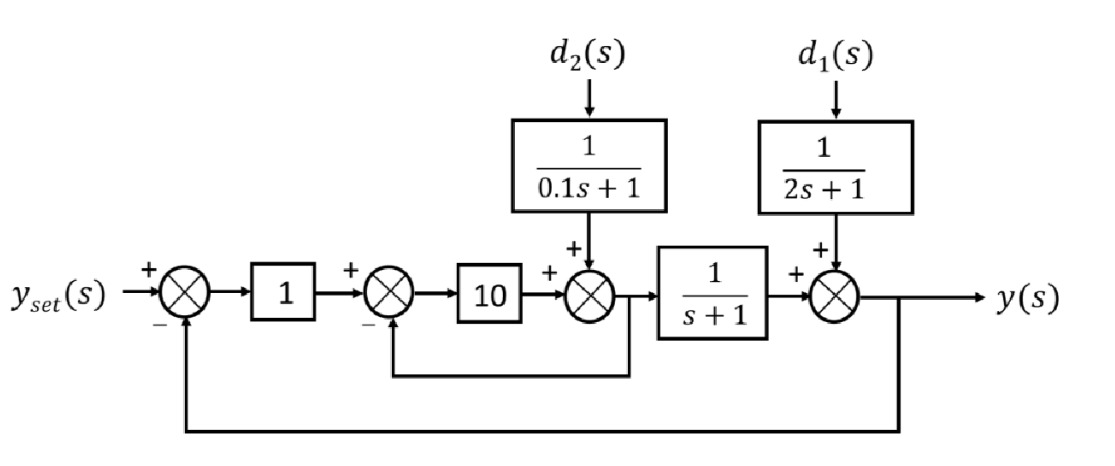
\includegraphics[scale=0.25]{2023/CH/44/figs/g44fig1.jpeg}
    \caption{ }
    \label{}
\end{figure}
\begin{enumerate}[label=\Alph*.]
\item $\frac{1}{(11s+21)(0.1s+1)}$ 
\item $\frac{1}{(s+1)(0.1s+1)}$
\item $\frac{(s+1)}{(s+2)(0.1s+1)}$
\item $\frac{(s+1)}{(s+1)(0.1s+1)}$
\end{enumerate} \hfill (GATE CH 2023)
\solution
\newpage
\item In the differential equation $\frac{dy}{dx} + \alpha x y = 0, \alpha$ is a positive constant. If $y = 1.0$ at
$x = 0.0$, and $y = 0.8$ at $x = 1.0$, the value of $\alpha$ is (rounded off to three decimal places).  \hfill(GATE CE 2023)
\solution

\newpage
\item The switch $S_1$ was closed and $S_2$ was open for a long time. At t=0,switch $S_1$ is opened and $S_2$ is closed,simultaneously. The value of $i_c(0^{+})$, in amperes, is . \hfill (GATE EC 2023)\\
\begin{circuitikz}[american]
   \draw (0,0) to [isource, l=1A] (0,4) ;
   \draw (0,0) to [short] (3,0) to [C = 0.01F] (3,4) to [short] (6,4) to [R = 100 $\Omega$] (6,2) to [L = 1H] (6,0) to [short] (9,0) to [R = 25 $\Omega$] (9,4) to [short] (6,4) ;
   \draw (3,0) to [short] (6,0) ;
   \draw (0,4) to [ospst = $S_1$] ++(3,0); 
   \draw (7.5,4) to [cspst = $S_2$] ++(0,-2);
   \draw (7.5,2) to [short] (6,2) ;
   \draw (3,4) to [short ,i = $i_c$] (3,3);
   
\end{circuitikz}

\newpage

\item The continuous time signal $x(t)$ is described by:
\begin{align}
x(t)=
    \begin{cases}
        1, & \text{if } 0\: {\displaystyle \leq }\:t\:{\displaystyle \leq }\:1\\
        0, & \text{elsewhere}
    \end{cases} 
\end{align}
If $y(t)$ represents $x(t)$ convolved with itself, which of the following options is/are TRUE?
\begin{enumerate}[label = \Alph*]
    \item $y(t)$ = 0 for all $t<0$\\
    \item $y(t)$ = 0 for all $t>1$\\
    \item $y(t)$ = 0 for all $t>3$\\
    \item $\int_{0.1}^{0.75} \frac{dy(t)}{dt}\: \text{dt} \neq 0$
\end{enumerate}
\solution
\newpage

\item The Z-transform of a discrete signal $x\brak{n}$ is
\begin{align}
X\brak{z}=\dfrac{4z}{\brak{z-\dfrac{1}{5}} \brak{z-\dfrac{2}{3}} \brak{z-3}} \text{ with ROC= }R
\end{align}
Which one of the following statements is TRUE?
\begin{enumerate}[label = (\alph*)]
     \item Discrete time Fourier transform of $x\sbrak{n}$ converges if $R$ is $|z|>3$\\
     \item Discrete time Fourier transform of $x\sbrak{n}$ converges if $ R$ is $\dfrac{2}{3}<|z|<3$\\
     \item Discrete time Fourier transform of $x\sbrak{n}$ converges if $R$ is such that $x\sbrak{n}$ is a left-sided sequence.\\
     \item Discrete time Fourier transform of $x\sbrak{n}$ converges if $R$ is such that $x\sbrak{n}$is a right-sided sequence.\\
 \end{enumerate} \hfill{GATE EE 2023}
 \solution
 \newpage
 
\item The phase margin of the transfer function $G(s) = \frac{2(1-s)}{(1+s)^2}$ is \rule{1cm}{0.15mm} degrees. (rounded off to the nearest integer). \hfill (GATE IN 2023)\\
\solution
\newpage
\item Consider the second-order linear differential equation
\[x^2\frac{d^2y}{dx^2}+x\frac{dy}{dx}-y=0, \; x\geq 1\]
with the initial conditions \[y(x=1)=6,\; \;\; \frac{dy}{dx}\big{|}_{x=1}=2.\]
Then the value of $y$ at $x=2$ is \rule{2cm}{0.1mm}.\\{\hfill{GATE ME 2023}}\\
\solution
\newpage
\item The transfer function of a measuring instrument is \\
$$G_m(s) = \frac{1.05}{2s+1}exp(-s)$$
At time $t = 0$, a step change of +1 unit is introduced in the input of this instrument.The time taken by the instrument to show an increase of 1 unit in its output is(rounded off to two decimal places).\\ \hfill (GATE CH 2023)
\solution
\item
The laplace transform of $x_1(t)$ = $e^{-t}u(t)$ is $X_1(s)$, where $u(t)$ is the unit step function. The laplace transform of $x_2(t) = e^tu(-t)$ is $X_2(s)$. Which one of the following statements is TRUE?
\begin{enumerate}
    \item The region of convergence of $X_1(s)$ is $Re(s) \geq 0$
    \item The region of convergence of $X_2(s)$ is confined to the left half-plane of s.
    \item The region of convergence of $X_1(s)$ is confined to the right half-plane of s.
    \item the imaginary axis in the s-plane is included in both the region of convergence of $X_1(s)$ and the region of convergence of $X_2(s)$.
\end{enumerate} \hfill(GATE BM 2023)\\
\solution
\newpage
\item Given that $\frac{dy}{dx}=2x+y$ and $y=1$,when $x=0$ Using Runge-Kutta fourth order method,the value of $y$ at $x=0.2$ is \hfill(GATE 2023 AG 50) \\
\solution

\item The magnitude and phase plots shown in the figure match with the transfer-
function
\begin{figure}[h]
    \centering
    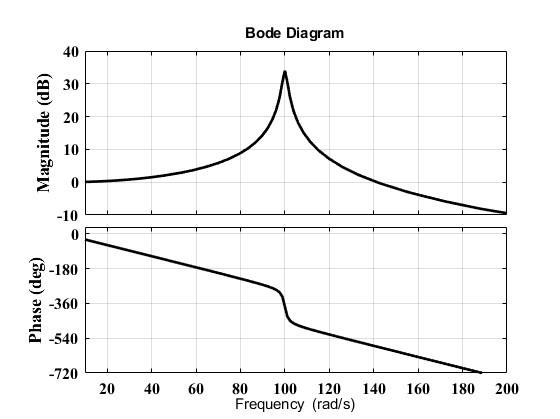
\includegraphics[width=\columnwidth]{2023/IN/43/figs/question.png}
\end{figure}\\
\begin{enumerate}
\item $\frac{10000}{s^2+2s+10000}$\\
\item $\frac{10000}{s^2+2s+10000}e^{-0.05s}$\\
\item $\frac{10000}{s^2+2s+10000}e^{-0.5\times10^{-12}s}$\\
\item $\frac{100}{s^2+2s+100}$
\end{enumerate}
\hfill{(GATE IN 2023)}
\solution

\newpage
\item The Laplace transform of the continuous-time signal $x\brak{t} = e^{-3t}u\brak{t - 5}$ is 
\rule{1cm}{0.15mm}, where $u\brak{t}$ denotes the continuous-time unit step signal.

\begin{enumerate}[label = \Alph*)]
    \item $\frac{e^{-5s}}{s + 3}$, Real$\{s\} > -3$\\
    \item $\frac{e^{-5(s - 3)}}{s - 3}$, Real$\{s\} > 3$\\
    \item $\frac{e^{-5(s + 3)}}{s + 3}$, Real$\{s\} > -3$\\
    \item $\frac{e^{-5(s - 3)}}{s + 3}$, Real$\{s\} > -3$\\
\end{enumerate}
\solution
\iffalse
\let\negmedspace\undefined
\let\negthickspace\undefined
\documentclass[journal,12pt,twocolumn]{IEEEtran}
\usepackage{cite}
\usepackage{amsmath,amssymb,amsfonts,amsthm}
\usepackage{algorithmic}
\usepackage{graphicx}
\usepackage{textcomp}
\usepackage{xcolor}
\usepackage{txfonts}
\usepackage{listings}
\usepackage{enumitem}
\usepackage{mathtools}
\usepackage{gensymb}
\usepackage{comment}
\usepackage[breaklinks=true]{hyperref}
\usepackage{tkz-euclide} 
\usepackage{listings}
\usepackage{gvv}                                        
\def\inputGnumericTable{}                                 
\usepackage[latin1]{inputenc}                                
\usepackage{color}                                            
\usepackage{array}                                            
\usepackage{longtable}                                       
\usepackage{calc}                                             
\usepackage{multirow}                                         
\usepackage{hhline}                                           
\usepackage{ifthen}                                           
\usepackage{lscape}
\usepackage[center]{caption} % center the captions to figure

\newtheorem{theorem}{Theorem}[section]
\newtheorem{problem}{Problem}
\newtheorem{proposition}{Proposition}[section]
\newtheorem{lemma}{Lemma}[section]
\newtheorem{corollary}[theorem]{Corollary}
\newtheorem{example}{Example}[section]
\newtheorem{definition}[problem]{Definition}
\newcommand{\BEQA}{\begin{eqnarray}}
\newcommand{\EEQA}{\end{eqnarray}}
\newcommand{\define}{\stackrel{\triangle}{=}}
\theoremstyle{remark}
\newtheorem{rem}{Remark}
\begin{document}

\newcolumntype{M}[1]{>{\centering\arraybackslash}m{#1}}
\newcolumntype{N}{@{}m{0pt}@{}}

\bibliographystyle{IEEEtran}
\vspace{3cm}

\title{GATE 2023 IN 37Q} 
\author{ee23btech11223 - Soham Prabhakar More% <-this % stops a space
}
\chapter{Laplace Transform}
\maketitle
\newpage
\bigskip

\renewcommand{\thefigure}{\theenumi}
\renewcommand{\thetable}{\theenumi}

\bibliographystyle{IEEEtran}

\question The Laplace transform of the continuous-time signal $x\brak{t} = e^{-3t}u\brak{t - 5}$ is 
\rule{1cm}{0.15mm}, where $u\brak{t}$ denotes the continuous-time unit step signal.

\solution
\fi

\begin{table}[ht]
    \begin{tabular}{|c|c|c|}
    \hline 
    \textbf{Parameter}&\textbf{Description} &\textbf{Value}\\
    \hline
    $x\brak{t}$ & Given Function & $x\brak{t} = e^{-3t}u\brak{t}$ \\
    \hline
	$X\brak{s}$ & Laplace Transform of $x\brak{t}$ & $\frac{e^{-5\brak{s + 3}}}{s + 3}$ \\
    \hline
\end{tabular}

\caption{Table of parameters}
\label{Table:1}


\end{table}    

\begin{align}
    e^{-3t}u\brak{t} \system{L} \frac{1}{s + 3} \quad \Re\brak{s} > -3 \label{eq:2023.in.37.exp}
\end{align}
Using time shifting,
\begin{align}
    e^{-3(t - 5)}u\brak{t - 5} &\system{L} \frac{e^{-5s}}{s + 3} \\
    e^{-15}e^{-3(t - 5)}u\brak{t - 5} &\system{L} e^{-15}\frac{e^{-5s}}{s + 3} \\
    e^{-3t}u\brak{t - 5} &\system{L} \frac{e^{-5(s + 3)}}{s + 3} \\
    \therefore x\brak{t} &\system{L} \frac{e^{-5(s + 3)}}{s + 3} \quad \Re\brak{s} > -3
\end{align}

\begin{figure}[h!]
    \renewcommand\thefigure{3}
    \centering
    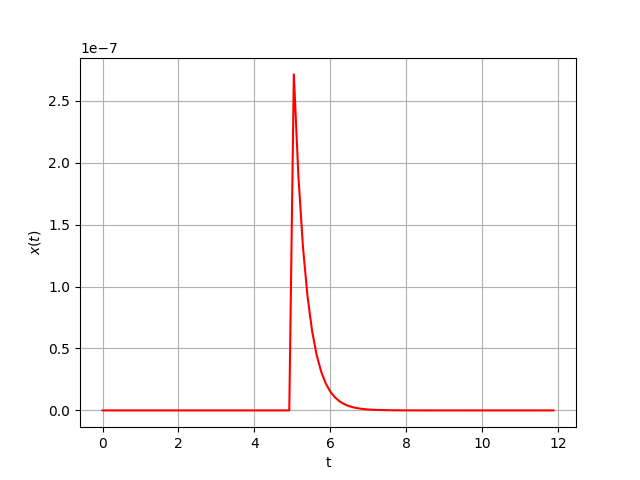
\includegraphics[width=\columnwidth]{2023/IN/37/figs/x_t.png}
    \caption[short]{Plot of $x\brak{t}$ vs $t$. See \tabref{Table:1}}
    \label{fig:2023.in.37.img1}
\end{figure}

%\end{document}



\newpage
\item The solution $ x(t) ,t \geq 0, $ to the differential equation
$ \ddot{x} = -k\dot{x}  , k > 0 $ with initial conditions $ x(0) = 1 $ and $ x\dot{o}(0) $ = 0 is\\
\solution
\pagebreak
\item  Consider the differential equation
\begin{align}
x^2\frac{d^2y}{dx^2} + 4x\frac{dy}{dx} + 2y = 0 \quad \text{for } x\geq 1 \nonumber
\end{align}
with initial conditions $y=0$ and $\frac{dy}{dx} = 1$ at
$x = 1$. The value of $y$ at $x = 2$ is ?\\

\hfill(GATE AE 2023)
\solution
\pagebreak
\item The Laplace transform of the continuous-time signal $x\brak{t} = e^{-3t}u\brak{t - 5}$ is 
\rule{1cm}{0.15mm}, where $u\brak{t}$ denotes the continuous-time unit step signal.


\solution
\iffalse
\let\negmedspace\undefined
\let\negthickspace\undefined
\documentclass[journal,12pt,twocolumn]{IEEEtran}
\usepackage{cite}
\usepackage{amsmath,amssymb,amsfonts,amsthm}
\usepackage{algorithmic}
\usepackage{graphicx}
\usepackage{textcomp}
\usepackage{xcolor}
\usepackage{txfonts}
\usepackage{listings}
\usepackage{enumitem}
\usepackage{mathtools}
\usepackage{gensymb}
\usepackage{comment}
\usepackage[breaklinks=true]{hyperref}
\usepackage{tkz-euclide} 
\usepackage{listings}
\usepackage{gvv}                                        
\def\inputGnumericTable{}                                 
\usepackage[latin1]{inputenc}                                
\usepackage{color}                                            
\usepackage{array}                                            
\usepackage{longtable}                                       
\usepackage{calc}                                             
\usepackage{multirow}                                         
\usepackage{hhline}                                           
\usepackage{ifthen}                                           
\usepackage{lscape}
\usepackage[center]{caption} % center the captions to figure

\newtheorem{theorem}{Theorem}[section]
\newtheorem{problem}{Problem}
\newtheorem{proposition}{Proposition}[section]
\newtheorem{lemma}{Lemma}[section]
\newtheorem{corollary}[theorem]{Corollary}
\newtheorem{example}{Example}[section]
\newtheorem{definition}[problem]{Definition}
\newcommand{\BEQA}{\begin{eqnarray}}
\newcommand{\EEQA}{\end{eqnarray}}
\newcommand{\define}{\stackrel{\triangle}{=}}
\theoremstyle{remark}
\newtheorem{rem}{Remark}
\begin{document}

\newcolumntype{M}[1]{>{\centering\arraybackslash}m{#1}}
\newcolumntype{N}{@{}m{0pt}@{}}

\bibliographystyle{IEEEtran}
\vspace{3cm}

\title{GATE 2023 IN 37Q} 
\author{ee23btech11223 - Soham Prabhakar More% <-this % stops a space
}
\chapter{Laplace Transform}
\maketitle
\newpage
\bigskip

\renewcommand{\thefigure}{\theenumi}
\renewcommand{\thetable}{\theenumi}

\bibliographystyle{IEEEtran}

\question The Laplace transform of the continuous-time signal $x\brak{t} = e^{-3t}u\brak{t - 5}$ is 
\rule{1cm}{0.15mm}, where $u\brak{t}$ denotes the continuous-time unit step signal.

\solution
\fi

\begin{table}[ht]
    \begin{tabular}{|c|c|c|}
    \hline 
    \textbf{Parameter}&\textbf{Description} &\textbf{Value}\\
    \hline
    $x\brak{t}$ & Given Function & $x\brak{t} = e^{-3t}u\brak{t}$ \\
    \hline
	$X\brak{s}$ & Laplace Transform of $x\brak{t}$ & $\frac{e^{-5\brak{s + 3}}}{s + 3}$ \\
    \hline
\end{tabular}

\caption{Table of parameters}
\label{Table:1}


\end{table}    

\begin{align}
    e^{-3t}u\brak{t} \system{L} \frac{1}{s + 3} \quad \Re\brak{s} > -3 \label{eq:2023.in.37.exp}
\end{align}
Using time shifting,
\begin{align}
    e^{-3(t - 5)}u\brak{t - 5} &\system{L} \frac{e^{-5s}}{s + 3} \\
    e^{-15}e^{-3(t - 5)}u\brak{t - 5} &\system{L} e^{-15}\frac{e^{-5s}}{s + 3} \\
    e^{-3t}u\brak{t - 5} &\system{L} \frac{e^{-5(s + 3)}}{s + 3} \\
    \therefore x\brak{t} &\system{L} \frac{e^{-5(s + 3)}}{s + 3} \quad \Re\brak{s} > -3
\end{align}

\begin{figure}[h!]
    \renewcommand\thefigure{3}
    \centering
    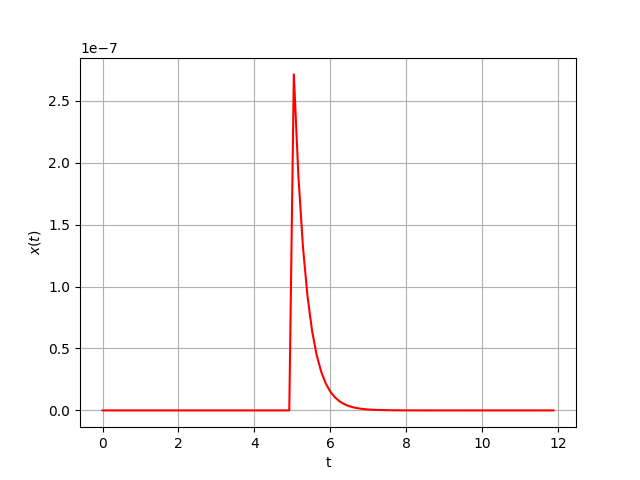
\includegraphics[width=\columnwidth]{2023/IN/37/figs/x_t.png}
    \caption[short]{Plot of $x\brak{t}$ vs $t$. See \tabref{Table:1}}
    \label{fig:2023.in.37.img1}
\end{figure}

%\end{document}



\newpage


\end{enumerate}